% Options for packages loaded elsewhere
\PassOptionsToPackage{unicode}{hyperref}
\PassOptionsToPackage{hyphens}{url}
%
\documentclass[
]{book}
\usepackage{lmodern}
\usepackage{amssymb,amsmath}
\usepackage{ifxetex,ifluatex}
\ifnum 0\ifxetex 1\fi\ifluatex 1\fi=0 % if pdftex
  \usepackage[T1]{fontenc}
  \usepackage[utf8]{inputenc}
  \usepackage{textcomp} % provide euro and other symbols
\else % if luatex or xetex
  \usepackage{unicode-math}
  \defaultfontfeatures{Scale=MatchLowercase}
  \defaultfontfeatures[\rmfamily]{Ligatures=TeX,Scale=1}
\fi
% Use upquote if available, for straight quotes in verbatim environments
\IfFileExists{upquote.sty}{\usepackage{upquote}}{}
\IfFileExists{microtype.sty}{% use microtype if available
  \usepackage[]{microtype}
  \UseMicrotypeSet[protrusion]{basicmath} % disable protrusion for tt fonts
}{}
\makeatletter
\@ifundefined{KOMAClassName}{% if non-KOMA class
  \IfFileExists{parskip.sty}{%
    \usepackage{parskip}
  }{% else
    \setlength{\parindent}{0pt}
    \setlength{\parskip}{6pt plus 2pt minus 1pt}}
}{% if KOMA class
  \KOMAoptions{parskip=half}}
\makeatother
\usepackage{xcolor}
\IfFileExists{xurl.sty}{\usepackage{xurl}}{} % add URL line breaks if available
\IfFileExists{bookmark.sty}{\usepackage{bookmark}}{\usepackage{hyperref}}
\hypersetup{
  pdftitle={DNA Hydroxymethylation in Hepatocellular Carcinoma},
  pdfauthor={Francois Collin},
  hidelinks,
  pdfcreator={LaTeX via pandoc}}
\urlstyle{same} % disable monospaced font for URLs
\usepackage{color}
\usepackage{fancyvrb}
\newcommand{\VerbBar}{|}
\newcommand{\VERB}{\Verb[commandchars=\\\{\}]}
\DefineVerbatimEnvironment{Highlighting}{Verbatim}{commandchars=\\\{\}}
% Add ',fontsize=\small' for more characters per line
\usepackage{framed}
\definecolor{shadecolor}{RGB}{248,248,248}
\newenvironment{Shaded}{\begin{snugshade}}{\end{snugshade}}
\newcommand{\AlertTok}[1]{\textcolor[rgb]{0.94,0.16,0.16}{#1}}
\newcommand{\AnnotationTok}[1]{\textcolor[rgb]{0.56,0.35,0.01}{\textbf{\textit{#1}}}}
\newcommand{\AttributeTok}[1]{\textcolor[rgb]{0.77,0.63,0.00}{#1}}
\newcommand{\BaseNTok}[1]{\textcolor[rgb]{0.00,0.00,0.81}{#1}}
\newcommand{\BuiltInTok}[1]{#1}
\newcommand{\CharTok}[1]{\textcolor[rgb]{0.31,0.60,0.02}{#1}}
\newcommand{\CommentTok}[1]{\textcolor[rgb]{0.56,0.35,0.01}{\textit{#1}}}
\newcommand{\CommentVarTok}[1]{\textcolor[rgb]{0.56,0.35,0.01}{\textbf{\textit{#1}}}}
\newcommand{\ConstantTok}[1]{\textcolor[rgb]{0.00,0.00,0.00}{#1}}
\newcommand{\ControlFlowTok}[1]{\textcolor[rgb]{0.13,0.29,0.53}{\textbf{#1}}}
\newcommand{\DataTypeTok}[1]{\textcolor[rgb]{0.13,0.29,0.53}{#1}}
\newcommand{\DecValTok}[1]{\textcolor[rgb]{0.00,0.00,0.81}{#1}}
\newcommand{\DocumentationTok}[1]{\textcolor[rgb]{0.56,0.35,0.01}{\textbf{\textit{#1}}}}
\newcommand{\ErrorTok}[1]{\textcolor[rgb]{0.64,0.00,0.00}{\textbf{#1}}}
\newcommand{\ExtensionTok}[1]{#1}
\newcommand{\FloatTok}[1]{\textcolor[rgb]{0.00,0.00,0.81}{#1}}
\newcommand{\FunctionTok}[1]{\textcolor[rgb]{0.00,0.00,0.00}{#1}}
\newcommand{\ImportTok}[1]{#1}
\newcommand{\InformationTok}[1]{\textcolor[rgb]{0.56,0.35,0.01}{\textbf{\textit{#1}}}}
\newcommand{\KeywordTok}[1]{\textcolor[rgb]{0.13,0.29,0.53}{\textbf{#1}}}
\newcommand{\NormalTok}[1]{#1}
\newcommand{\OperatorTok}[1]{\textcolor[rgb]{0.81,0.36,0.00}{\textbf{#1}}}
\newcommand{\OtherTok}[1]{\textcolor[rgb]{0.56,0.35,0.01}{#1}}
\newcommand{\PreprocessorTok}[1]{\textcolor[rgb]{0.56,0.35,0.01}{\textit{#1}}}
\newcommand{\RegionMarkerTok}[1]{#1}
\newcommand{\SpecialCharTok}[1]{\textcolor[rgb]{0.00,0.00,0.00}{#1}}
\newcommand{\SpecialStringTok}[1]{\textcolor[rgb]{0.31,0.60,0.02}{#1}}
\newcommand{\StringTok}[1]{\textcolor[rgb]{0.31,0.60,0.02}{#1}}
\newcommand{\VariableTok}[1]{\textcolor[rgb]{0.00,0.00,0.00}{#1}}
\newcommand{\VerbatimStringTok}[1]{\textcolor[rgb]{0.31,0.60,0.02}{#1}}
\newcommand{\WarningTok}[1]{\textcolor[rgb]{0.56,0.35,0.01}{\textbf{\textit{#1}}}}
\usepackage{longtable,booktabs}
% Correct order of tables after \paragraph or \subparagraph
\usepackage{etoolbox}
\makeatletter
\patchcmd\longtable{\par}{\if@noskipsec\mbox{}\fi\par}{}{}
\makeatother
% Allow footnotes in longtable head/foot
\IfFileExists{footnotehyper.sty}{\usepackage{footnotehyper}}{\usepackage{footnote}}
\makesavenoteenv{longtable}
\usepackage{graphicx}
\makeatletter
\def\maxwidth{\ifdim\Gin@nat@width>\linewidth\linewidth\else\Gin@nat@width\fi}
\def\maxheight{\ifdim\Gin@nat@height>\textheight\textheight\else\Gin@nat@height\fi}
\makeatother
% Scale images if necessary, so that they will not overflow the page
% margins by default, and it is still possible to overwrite the defaults
% using explicit options in \includegraphics[width, height, ...]{}
\setkeys{Gin}{width=\maxwidth,height=\maxheight,keepaspectratio}
% Set default figure placement to htbp
\makeatletter
\def\fps@figure{htbp}
\makeatother
\setlength{\emergencystretch}{3em} % prevent overfull lines
\providecommand{\tightlist}{%
  \setlength{\itemsep}{0pt}\setlength{\parskip}{0pt}}
\setcounter{secnumdepth}{5}
\usepackage{booktabs}
\usepackage[]{natbib}
\bibliographystyle{plainnat}

\title{DNA Hydroxymethylation in Hepatocellular Carcinoma}
\author{Francois Collin}
\date{2020-08-25}

\begin{document}
\maketitle

{
\setcounter{tocdepth}{1}
\tableofcontents
}
\hypertarget{index}{%
\chapter*{Preamble}\label{index}}
\addcontentsline{toc}{chapter}{Preamble}

This vignette offers some exploratory data analyses of data available from
the \href{https://www.ncbi.nlm.nih.gov/geo/}{NCBI GEO web site}.

\hypertarget{license}{%
\section*{License}\label{license}}
\addcontentsline{toc}{section}{License}


\includegraphics{CC_4_0.png}

This work by Francois Collin is licensed under a
\href{http://creativecommons.org/licenses/by/4.0/}{Creative Commons Attribution 4.0 International License}

\hypertarget{intro}{%
\chapter{Introduction}\label{intro}}

The goal of detecting
cancer at the earliest stage of development with a non-invasive procedure
has busied many groups with the task of perfecting techniques to support
what has become commonly known as a
liquid biopsy - the analysis of biomarkers circulating in fluids such as blood,
saliva or urine. Epigenetic biomarkers present themselves as good candidates for this application
(Gai and Sun (2019) \citep{Gai:2019aa}). In particular,
given their prevalence in the human genome,
close correlation with gene expression and high chemical stability,
DNA modifications such as 5-methylcytosine (5mC) and 5-hydroxymethylcytosine (5hmC)
are DNA epigenetic marks that provide much promise as
cancer diagnosis biomarkers that could be profitably analyzed in liquid biopsies
\citep{Cai:2019aa, Li:2017aa, Song:2017aa, Collin:2018aa}.

Li et al.~(2017) \citep{Li:2017aa} used a sensitive and selective chemical labeling technology
to extract genome-wide 5hmC profiles from circulating cell-free DNA (cfDNA)
as well as from genomic DNA (gDNA)
collected from a cohort of 260 patients recently diagnosed with colorectal,
gastric, pancreatic, liver or thyroid cancer and normal tissues from 90 healthy individuals
They found 5hmC-based biomarkers of circulating cfDNA to be highly predictive of some cancer types.
Similar small sample size findings were reported in Song et al.~(2017) \citep{Song:2017aa}.

Focusing on hepatocellular carcinoma, Cai et al.~(2019) \citep{Cai:2019aa} assembled a sizable dataset
to demonstrate the feasibility of using features derived from
5-hydroxymethylcytosines marks in circulating cell-free DNA as
a non-invasive approach for the early detection of
hepatocellular carcinoma. The data that are the basis of that
report are available on the NCBI GEO web site
(\href{https://www.ncbi.nlm.nih.gov/geo/query/acc.cgi?acc=GSE112679}{Series GSE112679}).
The data have also been bundled in a R data package which can be installed from github:

\begin{verbatim}
if (!requireNamespace("devtools", quietly = TRUE))
    install.packages("devtools")
devtools::install_github("12379Monty/GSE112679")
\end{verbatim}

An important question in the early development of classifiers of the sorts
that are the basis of any liquid biopsy diagnostic tool is how many samples
should be collected to make properly informed decisions. In this
report we will explore the GSE112679 data to shed some light on
the relationship between sample size and model performance
in the context classifying samples based on 5hmC data.

In Section \ref{preproc} we preprocess the data that
we will use for the classification analysis and perform some light QC analyses.
In Section \ref{baseline-model} we fit some models to discriminate between
early stage HCC and control samples and examine their performance.
In Section \ref{model-suite} we examine the results of fitting a suite of models to
investigate the effect of sample size on model performance.

\hypertarget{preproc}{%
\chapter{Preprocessing}\label{preproc}}

\hypertarget{load-the-data}{%
\section{Load the data}\label{load-the-data}}

The data that are available from NCBI GEO
\href{https://www.ncbi.nlm.nih.gov/geo/query/acc.cgi?acc=GSE112679}{Series GSE112679}
can be conveniently accessed through an R data package.
Attaching the GSE112679 package makes the count data tables
available as well as a gene annotation table and a sample description table.
See \href{https://12379monty.github.io/GSE112679/}{GSE112679 R Data Package page}.
For the Cai et al.~\citep{Cai:2019aa} model fitting and analysis, samples were separated into
\texttt{Train} and \texttt{Val-1} subsets. \texttt{Val-2} was an external validation set.

\begin{Shaded}
\begin{Highlighting}[]
\ControlFlowTok{if}\NormalTok{ (}\OperatorTok{!}\NormalTok{(}\StringTok{"GSE112679"} \OperatorTok{\%in\%}\StringTok{ }\KeywordTok{rownames}\NormalTok{(}\KeywordTok{installed.packages}\NormalTok{()))) \{}
  \ControlFlowTok{if}\NormalTok{ (}\OperatorTok{!}\KeywordTok{requireNamespace}\NormalTok{(}\StringTok{"devtools"}\NormalTok{, }\DataTypeTok{quietly =} \OtherTok{TRUE}\NormalTok{)) \{}
    \KeywordTok{install.packages}\NormalTok{(}\StringTok{"devtools"}\NormalTok{)}
\NormalTok{  \}}
\NormalTok{  devtools}\OperatorTok{::}\KeywordTok{install\_github}\NormalTok{(}\StringTok{"12379Monty/GSE112679"}\NormalTok{)}
\NormalTok{\}}
\KeywordTok{library}\NormalTok{(GSE112679)}
\KeywordTok{with}\NormalTok{(}
\NormalTok{  sampDesc }\OperatorTok{\%>\%}\StringTok{ }\NormalTok{dplyr}\OperatorTok{::}\KeywordTok{filter}\NormalTok{(sampType }\OperatorTok{==}\StringTok{ "blood"}\NormalTok{),}
  \KeywordTok{table}\NormalTok{(outcome, trainValGroup, }\DataTypeTok{exclude =} \OtherTok{NULL}\NormalTok{)}
\NormalTok{)}
\end{Highlighting}
\end{Shaded}

\begin{verbatim}
##            trainValGroup
## outcome     Train Val-1 Val-2
##   Benign      253   132     3
##   CHB         190    96     0
##   Cirrhosis    73    33     0
##   HCC         335   809    60
##   Healthy     269   124   177
\end{verbatim}

For this analysis, we will consider early stage cancer samples
and healthy or benign samples from the \texttt{Train} or \texttt{Val-1} subsets.

\begin{Shaded}
\begin{Highlighting}[]
\NormalTok{sampDescA <{-}}
\StringTok{  }\NormalTok{sampDesc }\OperatorTok{\%>\%}
\StringTok{  }\NormalTok{dplyr}\OperatorTok{::}\KeywordTok{filter}\NormalTok{(sampType }\OperatorTok{==}\StringTok{ "blood"} \OperatorTok{\&}\StringTok{ }\NormalTok{(trainValGroup }\OperatorTok{\%in\%}\StringTok{ }\KeywordTok{c}\NormalTok{(}\StringTok{"Train"}\NormalTok{, }\StringTok{"Val{-}1"}\NormalTok{)) }\OperatorTok{\&}
\StringTok{    }\NormalTok{((outcome2 }\OperatorTok{==}\StringTok{ "BenignHealthy"}\NormalTok{) }\OperatorTok{|}\StringTok{ }
\StringTok{     }\NormalTok{(outcome2 }\OperatorTok{==}\StringTok{ "HCC"} \OperatorTok{\&}\StringTok{ }\NormalTok{stage }\OperatorTok{==}\StringTok{ "Early"}\NormalTok{))) }\OperatorTok{\%>\%}
\StringTok{  }\NormalTok{dplyr}\OperatorTok{::}\KeywordTok{rename}\NormalTok{(}\DataTypeTok{group =}\NormalTok{ outcome2) }\OperatorTok{\%>\%}
\StringTok{  }\NormalTok{dplyr}\OperatorTok{::}\KeywordTok{arrange}\NormalTok{(group, sampID)}
\CommentTok{\# Recode group}
\NormalTok{sampDescA}\OperatorTok{$}\NormalTok{group <{-}}\StringTok{ }\KeywordTok{with}\NormalTok{(sampDescA, }
   \KeywordTok{ifelse}\NormalTok{(group }\OperatorTok{==}\StringTok{ "BenignHealthy"}\NormalTok{, }\StringTok{"Control"}\NormalTok{, group))}
\CommentTok{\# set groupCol for later}
\NormalTok{groupCol <{-}}\StringTok{ }\KeywordTok{c}\NormalTok{(}\StringTok{"\#F3C300"}\NormalTok{, }\StringTok{"\#875692"}\NormalTok{)}
\KeywordTok{names}\NormalTok{(groupCol) <{-}}\StringTok{ }\KeywordTok{unique}\NormalTok{(sampDescA}\OperatorTok{$}\NormalTok{group)}

\KeywordTok{with}\NormalTok{(sampDescA, }\KeywordTok{table}\NormalTok{(group, }\DataTypeTok{exclude =} \OtherTok{NULL}\NormalTok{))}
\end{Highlighting}
\end{Shaded}

\begin{verbatim}
## group
## Control     HCC 
##     778     555
\end{verbatim}

The features are counts of reads captured by chemical labeling, and indicate
the level of 5-hydroxymethylcytosines within each gene body. Cai et al.~(2019),
Li et al.~(2017) and Song et al.~(2017) \citep{Cai:2019aa, Li:2017aa, Song:2017aa}
all analyze 5hmC gene body counts using standard RNA-Seq methodologies, and we will
do the same here.

Note that before conducting any substantive analyses, the data would normally
be very carefully examined for any sign of quality variation between groups
of samples. This analysis would integrate sample meta data - where and when were
the blood samples collected - as well as library preparation and sequencing metrics
in order to detect any sign of processing artifacts that may be present in the dataset.
This is particularly important when dealing with blood samples as variable
DNA quality degradation is a well known challenge that is encountered when dealing with
such samples \citep{Huang:2017aa}. Although blood specimen handling protocols can be
put in place to minimize quality variation \citep{Permenter:2015aa}, variability
can never be completely eradicated, especially in the context of blood samples
collected by different groups, working in different environments. The problem
of variable DNA quality becomes paricularly pernicuous when it is compounded
with a confounding factor that sneaks in when the control sample collection
events are separated in time and space from the cancer sample collection events;
an all too common occurence.

As proper data QC requires an intimate familiarity with the details of
data collection and processing, such a task cannot be untertaken here.
We will simply run a \emph{minimal set of QC sanity checks} to make sure that
there are no apparent systematic effects in the data.

\begin{Shaded}
\begin{Highlighting}[]
 \CommentTok{\# Note that unique sample identifier are stored }
 \CommentTok{\# in the rownames of the sample description table }
 \CommentTok{\# and in the column names of the feature count tables.}
\NormalTok{  featureCountsA <{-}}\StringTok{ }\KeywordTok{cbind}\NormalTok{(Train\_featureCount, }
\NormalTok{                          Val1\_featureCount, }
\NormalTok{                          Val2\_featureCount)[,}\KeywordTok{rownames}\NormalTok{(sampDescA)]}
\end{Highlighting}
\end{Shaded}

We first look at coverage - make sure there isn't too much disparity of coverage
across samples. To detect shared variability, samples can be annotated and ordered
according to sample features that may be linked to sample batch processing. Here we
the samples have been ordered by group and sample id (an alias of geoAcc).

\begin{Shaded}
\begin{Highlighting}[]
\KeywordTok{par}\NormalTok{(}\DataTypeTok{mar =} \KeywordTok{c}\NormalTok{(}\DecValTok{1}\NormalTok{, }\DecValTok{3}\NormalTok{, }\DecValTok{2}\NormalTok{, }\DecValTok{1}\NormalTok{))}
\KeywordTok{boxplot}\NormalTok{(}\KeywordTok{log2}\NormalTok{(featureCountsA }\OperatorTok{+}\StringTok{ }\DecValTok{1}\NormalTok{),}
  \DataTypeTok{ylim =} \KeywordTok{c}\NormalTok{(}\DecValTok{3}\NormalTok{, }\DecValTok{11}\NormalTok{),}
  \DataTypeTok{staplewex =} \DecValTok{0}\NormalTok{,       }\CommentTok{\# remove horizontal whisker lines}
  \DataTypeTok{staplecol =} \StringTok{"white"}\NormalTok{, }\CommentTok{\# just to be totally sure :)}
  \DataTypeTok{outline =}\NormalTok{ F,         }\CommentTok{\# remove outlying points}
  \DataTypeTok{whisklty =} \DecValTok{0}\NormalTok{,        }\CommentTok{\# remove vertical whisker lines}
  \DataTypeTok{las =} \DecValTok{2}\NormalTok{, }\DataTypeTok{horizontal =}\NormalTok{ F, }\DataTypeTok{xaxt =} \StringTok{"n"}\NormalTok{,}
  \DataTypeTok{border =}\NormalTok{ groupCol[sampDescA}\OperatorTok{$}\NormalTok{group]}
\NormalTok{)}
\KeywordTok{legend}\NormalTok{(}\StringTok{"top"}\NormalTok{, }\DataTypeTok{legend =} \KeywordTok{names}\NormalTok{(groupCol), }\DataTypeTok{text.col =}\NormalTok{ groupCol, }
  \DataTypeTok{ncol =} \DecValTok{2}\NormalTok{, }\DataTypeTok{bty =} \StringTok{"n"}\NormalTok{)}
\CommentTok{\# Add reference lines}
\NormalTok{SampleMedian <{-}}\StringTok{ }\KeywordTok{apply}\NormalTok{(}\KeywordTok{log2}\NormalTok{(featureCountsA }\OperatorTok{+}\StringTok{ }\DecValTok{1}\NormalTok{), }\DecValTok{2}\NormalTok{, median)}
\KeywordTok{abline}\NormalTok{(}\DataTypeTok{h =} \KeywordTok{median}\NormalTok{(SampleMedian), }\DataTypeTok{col =} \StringTok{"grey"}\NormalTok{)}
\KeywordTok{axis}\NormalTok{(}\DataTypeTok{side =} \DecValTok{2}\NormalTok{, }\DataTypeTok{at =} \KeywordTok{round}\NormalTok{(}\KeywordTok{median}\NormalTok{(SampleMedian), }\DecValTok{1}\NormalTok{), }
  \DataTypeTok{las =} \DecValTok{2}\NormalTok{, }\DataTypeTok{col =} \StringTok{"grey"}\NormalTok{, }\DataTypeTok{line =} \DecValTok{{-}1}\NormalTok{, }\DataTypeTok{tick =}\NormalTok{ F)}
\end{Highlighting}
\end{Shaded}

\begin{figure}
\centering
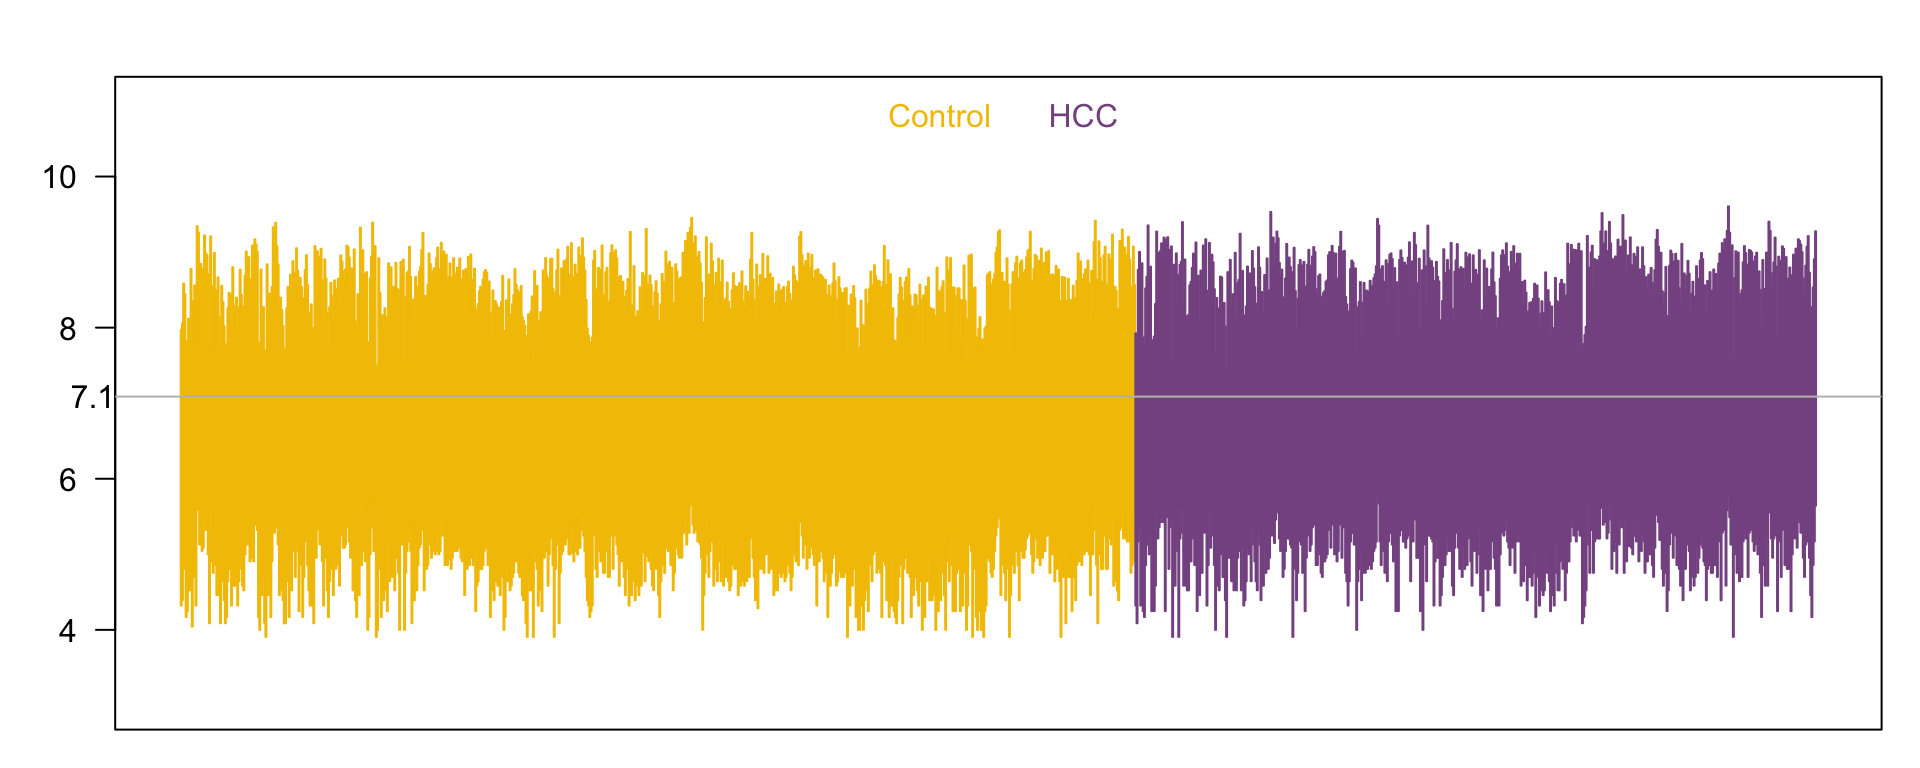
\includegraphics{HCC5hmCExplore_files/figure-latex/coverage-1.pdf}
\caption{\label{fig:coverage}Sample log2 count boxplots}
\end{figure}

We nest look at relative log representation (RLR) (in the context of measuring the density of
5hmC marks in genes, we refer to \texttt{representation} as opposed to \texttt{expression}; the
two can be used interchangibly) -
make sure the shapes of the distributions are not widely different.

\begin{Shaded}
\begin{Highlighting}[]
\NormalTok{lcpm\_mtx <{-}}\StringTok{ }\NormalTok{edgeR}\OperatorTok{::}\KeywordTok{cpm}\NormalTok{(featureCountsA, }\DataTypeTok{log =}\NormalTok{ T)}
\NormalTok{median\_vec <{-}}\StringTok{ }\KeywordTok{apply}\NormalTok{(lcpm\_mtx, }\DecValTok{1}\NormalTok{, median)}
\NormalTok{RLR\_mtx <{-}}\StringTok{ }\KeywordTok{sweep}\NormalTok{(lcpm\_mtx, }\DecValTok{1}\NormalTok{, median\_vec, }\StringTok{"{-}"}\NormalTok{)}

\KeywordTok{par}\NormalTok{(}\DataTypeTok{mar =} \KeywordTok{c}\NormalTok{(}\DecValTok{1}\NormalTok{, }\DecValTok{3}\NormalTok{, }\DecValTok{2}\NormalTok{, }\DecValTok{1}\NormalTok{))}
\KeywordTok{boxplot}\NormalTok{(RLR\_mtx,}
  \DataTypeTok{xlab =} \StringTok{""}\NormalTok{, }\DataTypeTok{ylim =} \KeywordTok{c}\NormalTok{(}\OperatorTok{{-}}\NormalTok{.}\DecValTok{6}\NormalTok{, }\FloatTok{.6}\NormalTok{),}
  \DataTypeTok{staplewex =} \DecValTok{0}\NormalTok{, }\CommentTok{\# remove horizontal whisker lines}
  \DataTypeTok{staplecol =} \StringTok{"white"}\NormalTok{, }\CommentTok{\# just to be totally sure :)}
  \DataTypeTok{outline =}\NormalTok{ F, }\CommentTok{\# remove outlying points}
  \DataTypeTok{whisklty =} \DecValTok{0}\NormalTok{, }\CommentTok{\# remove vertical whisker lines}
  \DataTypeTok{las =} \DecValTok{2}\NormalTok{, }\DataTypeTok{horizontal =}\NormalTok{ F, }\DataTypeTok{xaxt =} \StringTok{"n"}\NormalTok{,}
  \DataTypeTok{border =}\NormalTok{ groupCol[sampDescA}\OperatorTok{$}\NormalTok{group]}
\NormalTok{)}
\KeywordTok{legend}\NormalTok{(}\StringTok{"top"}\NormalTok{, }\DataTypeTok{legend =} \KeywordTok{names}\NormalTok{(groupCol), }
  \DataTypeTok{text.col =}\NormalTok{ groupCol, }\DataTypeTok{ncol =} \DecValTok{2}\NormalTok{, }\DataTypeTok{bty =} \StringTok{"n"}\NormalTok{)}
\CommentTok{\# Add group Q1, Q3}
\ControlFlowTok{for}\NormalTok{ (GRP }\ControlFlowTok{in} \KeywordTok{unique}\NormalTok{(sampDescA}\OperatorTok{$}\NormalTok{group)) \{}
\NormalTok{  group\_ndx <{-}}\StringTok{ }\KeywordTok{which}\NormalTok{(sampDescA}\OperatorTok{$}\NormalTok{group }\OperatorTok{==}\StringTok{ }\NormalTok{GRP)}
\NormalTok{  group\_Q1Q3\_mtx <{-}}\StringTok{ }\KeywordTok{apply}\NormalTok{(RLR\_mtx[, group\_ndx], }\DecValTok{2}\NormalTok{, }
\NormalTok{     quantile, }\DataTypeTok{prob =} \KeywordTok{c}\NormalTok{(.}\DecValTok{25}\NormalTok{, }\FloatTok{.75}\NormalTok{))}
  \KeywordTok{abline}\NormalTok{(}\DataTypeTok{h =} \KeywordTok{apply}\NormalTok{(group\_Q1Q3\_mtx, }\DecValTok{1}\NormalTok{, median), }
     \DataTypeTok{col =}\NormalTok{ groupCol[GRP], }\DataTypeTok{lwd =} \DecValTok{2}\NormalTok{)}
\NormalTok{\}}
\end{Highlighting}
\end{Shaded}

\begin{figure}
\centering
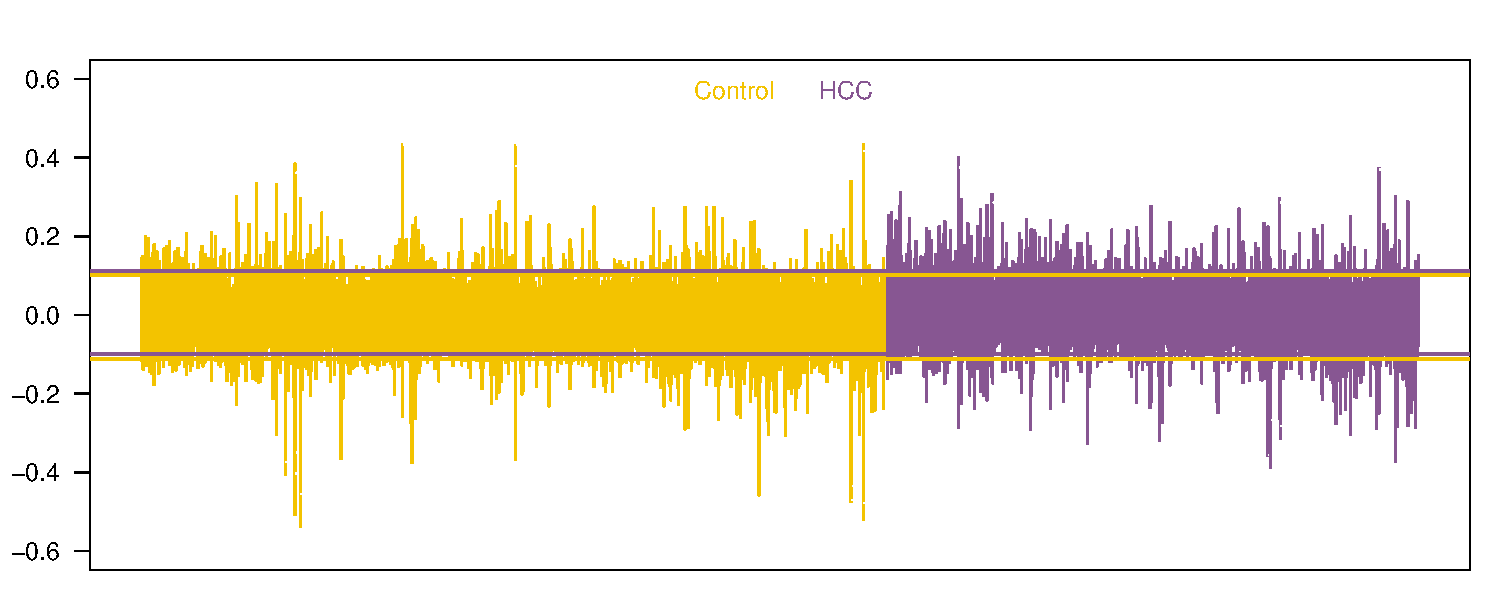
\includegraphics{HCC5hmCExplore_files/figure-latex/rlr-1.pdf}
\caption{\label{fig:rlr}Sample RLR}
\end{figure}

We note that the HCC samples have slightly more variable coverage distribution.
A few samples are quite different.

\hypertarget{normalized-representation-feature---log_2-cpm}{%
\section{\texorpdfstring{Normalized representation feature - \(log_2\) CPM}{Normalized representation feature - log\_2 CPM}}\label{normalized-representation-feature---log_2-cpm}}

We will use \(log_2\) normalized counts per million as our indicator
of 5hmC gene representation in our downstream analyses.
We will first remove weakly represented genes, as is typically done when
analyzing RNA-Seq data \citep{Law:2018aa}. Before removing genes, let's examine the
shapes of the distributions.

\begin{Shaded}
\begin{Highlighting}[]
\KeywordTok{par}\NormalTok{(}\DataTypeTok{mar =} \KeywordTok{c}\NormalTok{(}\DecValTok{3}\NormalTok{, }\DecValTok{3}\NormalTok{, }\DecValTok{2}\NormalTok{, }\DecValTok{1}\NormalTok{))}
\KeywordTok{plot}\NormalTok{(}\KeywordTok{density}\NormalTok{(lcpm\_mtx[, }\DecValTok{1}\NormalTok{]),}
  \DataTypeTok{col =}\NormalTok{ groupCol[sampDescA}\OperatorTok{$}\NormalTok{group[}\DecValTok{1}\NormalTok{]],}
  \DataTypeTok{lwd =} \DecValTok{2}\NormalTok{, }\DataTypeTok{ylim =} \KeywordTok{c}\NormalTok{(}\DecValTok{0}\NormalTok{, }\FloatTok{.25}\NormalTok{), }\DataTypeTok{las =} \DecValTok{2}\NormalTok{, }\DataTypeTok{main =} \StringTok{""}\NormalTok{, }\DataTypeTok{xlab =} \StringTok{""}
\NormalTok{)}
\KeywordTok{abline}\NormalTok{(}\DataTypeTok{v =} \DecValTok{0}\NormalTok{, }\DataTypeTok{col =} \DecValTok{3}\NormalTok{)}
\CommentTok{\# After verifying no outliers, can plot a random subset }
\ControlFlowTok{for}\NormalTok{ (JJ }\ControlFlowTok{in} \KeywordTok{sample}\NormalTok{(}\DecValTok{2}\OperatorTok{:}\KeywordTok{ncol}\NormalTok{(lcpm\_mtx), }\DataTypeTok{size =} \DecValTok{100}\NormalTok{)) \{}
\NormalTok{  den <{-}}\StringTok{ }\KeywordTok{density}\NormalTok{(lcpm\_mtx[, JJ])}
  \KeywordTok{lines}\NormalTok{(den}\OperatorTok{$}\NormalTok{x, den}\OperatorTok{$}\NormalTok{y, }\DataTypeTok{col =}\NormalTok{ groupCol[sampDescA}\OperatorTok{$}\NormalTok{group[JJ]], }\DataTypeTok{lwd =} \DecValTok{2}\NormalTok{)}
\NormalTok{\} }\CommentTok{\# for(JJ}
\KeywordTok{legend}\NormalTok{(}\StringTok{"topright"}\NormalTok{, }\DataTypeTok{legend =} \KeywordTok{names}\NormalTok{(groupCol), }
  \DataTypeTok{text.col =}\NormalTok{ groupCol, }\DataTypeTok{bty =} \StringTok{"n"}\NormalTok{)}
\end{Highlighting}
\end{Shaded}

\begin{figure}
\centering
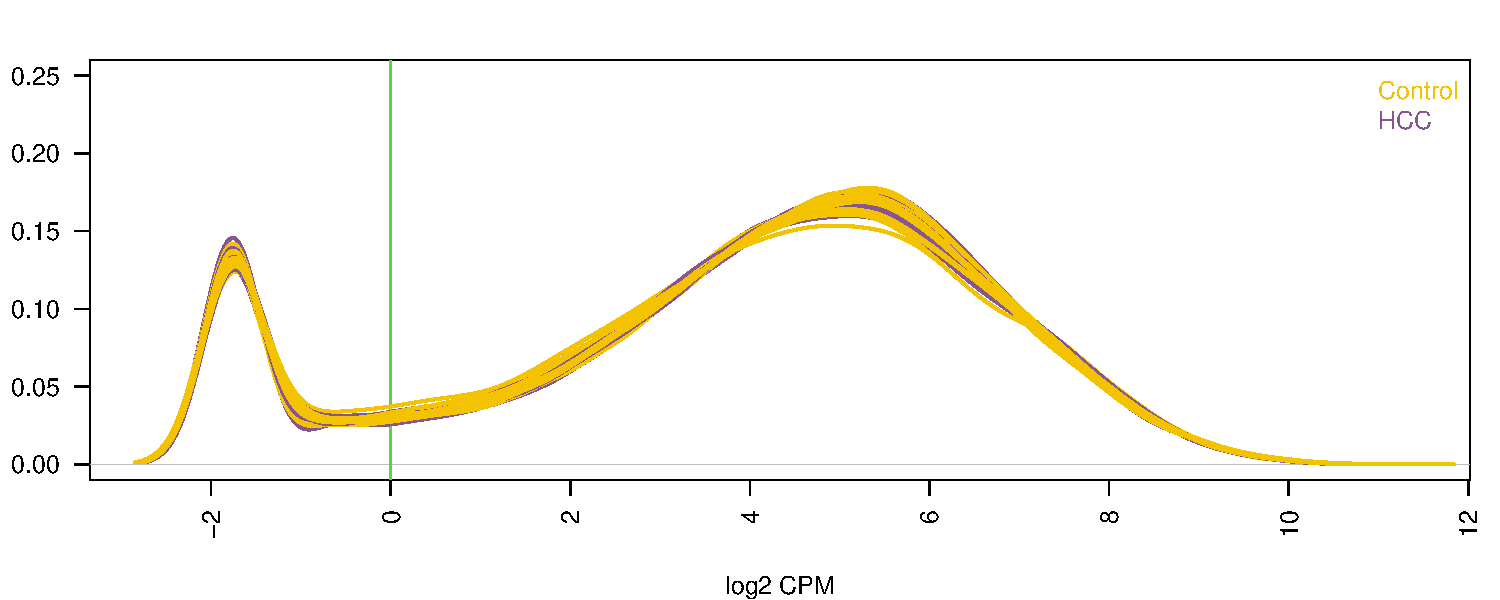
\includegraphics{HCC5hmCExplore_files/figure-latex/densityLcpm-1.pdf}
\caption{\label{fig:densityLcpm}Sample \(log_2\) CPM densities}
\end{figure}

We notice many weakly represented genes as is the case with RNA-Seq data.
Law et al.~(2018) \citep{Law:2018aa} point out that genes that are not expressed at a biologically
meaningful level in any condition should be discarded to reduce the
subset of genes to those that are of interest, and to reduce the number of tests
carried out downstream when looking at differential expression.

Using a nominal CPM value of 10, genes are deeemed to be \texttt{represented}
if their expression is above this threshold, and not represented otherwise.
Genes must be \texttt{represented} in at least 10 samples across the entire
dataset to be retained for downstream analysis. Here, a CPM value of 10
means that a gene is represented if it has at least 29
reads in the sample with the lowest sequencing depth
(library size 2.9 million). Note that the thresholds
used here are arbitrary as there are no hard and fast rules to set thes by.

Remove weakly represented genes.

Removing 28.1\% of genes\ldots{}

\begin{Shaded}
\begin{Highlighting}[]
\NormalTok{featureCountsA <{-}}\StringTok{ }\NormalTok{featureCountsA[}\OperatorTok{!}\NormalTok{weak\_flg, ]}
\NormalTok{genes\_annotA <{-}}\StringTok{ }\NormalTok{genes\_annot[}\KeywordTok{rownames}\NormalTok{(featureCountsA), ]}
\NormalTok{lcpm\_mtx <{-}}\StringTok{ }\NormalTok{edgeR}\OperatorTok{::}\KeywordTok{cpm}\NormalTok{(featureCountsA, }\DataTypeTok{log =}\NormalTok{ T)}
\KeywordTok{dim}\NormalTok{(lcpm\_mtx)}
\end{Highlighting}
\end{Shaded}

\begin{verbatim}
## [1] 13725  1333
\end{verbatim}

Replot densities after removing weak genes.

\begin{Shaded}
\begin{Highlighting}[]
\KeywordTok{par}\NormalTok{(}\DataTypeTok{mar =} \KeywordTok{c}\NormalTok{(}\DecValTok{3}\NormalTok{, }\DecValTok{3}\NormalTok{, }\DecValTok{2}\NormalTok{, }\DecValTok{1}\NormalTok{))}
\KeywordTok{plot}\NormalTok{(}\KeywordTok{density}\NormalTok{(lcpm\_mtx[, }\DecValTok{1}\NormalTok{]),}
  \DataTypeTok{col =}\NormalTok{ groupCol[sampDescA}\OperatorTok{$}\NormalTok{group[}\DecValTok{1}\NormalTok{]],}
  \DataTypeTok{lwd =} \DecValTok{2}\NormalTok{, }\DataTypeTok{ylim =} \KeywordTok{c}\NormalTok{(}\DecValTok{0}\NormalTok{, }\FloatTok{.25}\NormalTok{), }\DataTypeTok{las =} \DecValTok{2}\NormalTok{, }\DataTypeTok{main =} \StringTok{""}\NormalTok{, }\DataTypeTok{xlab =} \StringTok{""}
\NormalTok{)}
\KeywordTok{abline}\NormalTok{(}\DataTypeTok{v =} \DecValTok{0}\NormalTok{, }\DataTypeTok{col =} \DecValTok{3}\NormalTok{)}
\CommentTok{\# After verifying no outliers, can plot a random subset }
\ControlFlowTok{for}\NormalTok{ (JJ }\ControlFlowTok{in} \KeywordTok{sample}\NormalTok{(}\DecValTok{2}\OperatorTok{:}\KeywordTok{ncol}\NormalTok{(lcpm\_mtx), }\DataTypeTok{size =} \DecValTok{100}\NormalTok{)) \{}
\NormalTok{  den <{-}}\StringTok{ }\KeywordTok{density}\NormalTok{(lcpm\_mtx[, JJ])}
  \KeywordTok{lines}\NormalTok{(den}\OperatorTok{$}\NormalTok{x, den}\OperatorTok{$}\NormalTok{y, }\DataTypeTok{col =}\NormalTok{ groupCol[sampDescA}\OperatorTok{$}\NormalTok{group[JJ]], }\DataTypeTok{lwd =} \DecValTok{2}\NormalTok{)}
\NormalTok{\} }\CommentTok{\# for(JJ}
\KeywordTok{legend}\NormalTok{(}\StringTok{"topright"}\NormalTok{, }\DataTypeTok{legend =} \KeywordTok{names}\NormalTok{(groupCol), }
  \DataTypeTok{text.col =}\NormalTok{ groupCol, }\DataTypeTok{bty =} \StringTok{"n"}\NormalTok{)}
\end{Highlighting}
\end{Shaded}

\begin{figure}
\centering
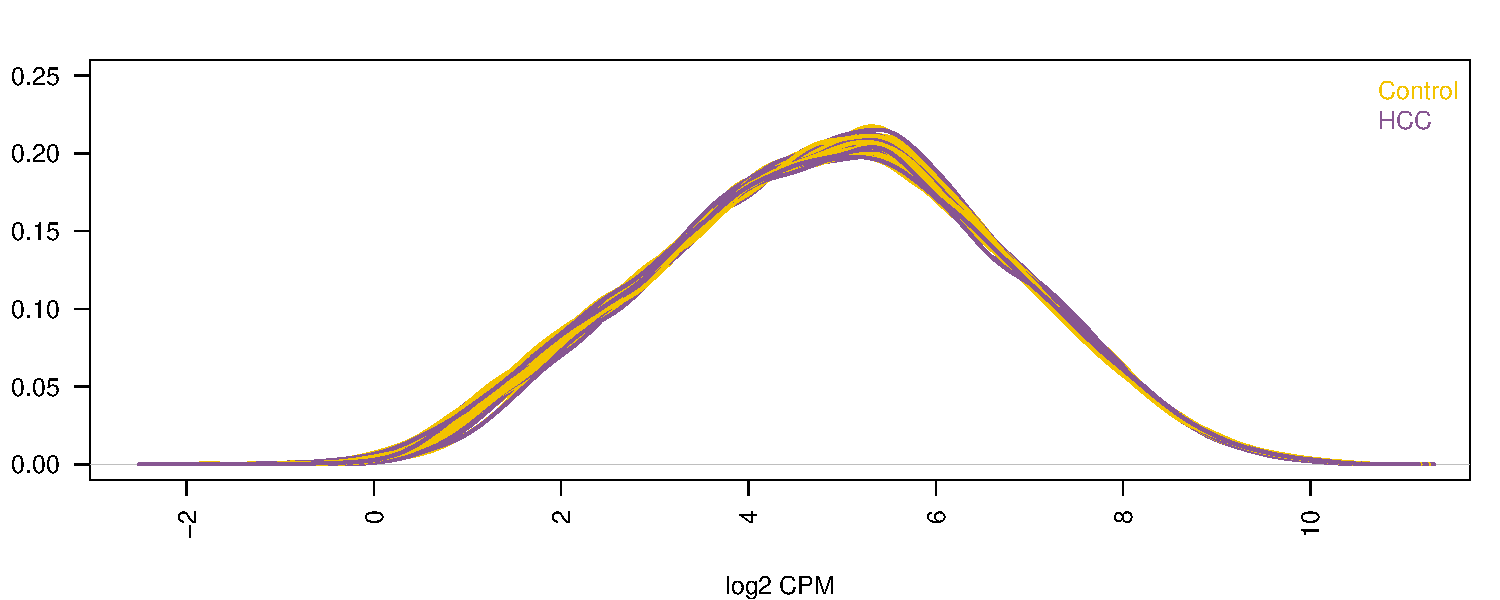
\includegraphics{HCC5hmCExplore_files/figure-latex/densityLcpm2-1.pdf}
\caption{\label{fig:densityLcpm2}Sample \(log_2\) CPM densities after removing weak genes}
\end{figure}

Note that the \(log_2(CMP)\) distribution is not quite symmetric.

As another sanity check, we will look at a
multidimensional scaling plot of distances between gene expression
profiles. We use \texttt{plotMDS} in limma package \citep{Ritchie:2015aa}),
which plots samples on a two-dimensional scatterplot so that distances on
the plot approximate the typical log2 fold changes between the
samples.

\begin{Shaded}
\begin{Highlighting}[]
 \KeywordTok{par}\NormalTok{(}\DataTypeTok{mfcol=}\KeywordTok{c}\NormalTok{(}\DecValTok{1}\NormalTok{,}\DecValTok{2}\NormalTok{), }\DataTypeTok{mar=}\KeywordTok{c}\NormalTok{(}\DecValTok{4}\NormalTok{,}\DecValTok{4}\NormalTok{,}\DecValTok{2}\NormalTok{,}\DecValTok{1}\NormalTok{), }\DataTypeTok{xpd=}\OtherTok{NA}\NormalTok{, }\DataTypeTok{oma=}\KeywordTok{c}\NormalTok{(}\DecValTok{0}\NormalTok{,}\DecValTok{0}\NormalTok{,}\DecValTok{2}\NormalTok{,}\DecValTok{0}\NormalTok{))}

\CommentTok{\# without loss of generality or sensitivity, sample 300 samples}
\CommentTok{\# this is simply a matter of convenience and to save time}
 \KeywordTok{set.seed}\NormalTok{(}\DecValTok{1}\NormalTok{)}
\NormalTok{ samp\_ndx <{-}}\StringTok{ }\KeywordTok{sample}\NormalTok{(}\DecValTok{1}\OperatorTok{:}\KeywordTok{ncol}\NormalTok{(lcpm\_mtx), }\DataTypeTok{size=}\DecValTok{500}\NormalTok{)}
\NormalTok{ MDS.out <{-}}\StringTok{ }\NormalTok{limma}\OperatorTok{::}\KeywordTok{plotMDS}\NormalTok{(lcpm\_mtx[,samp\_ndx], }
  \DataTypeTok{col=}\NormalTok{groupCol[sampDescA}\OperatorTok{$}\NormalTok{group[samp\_ndx]], }\DataTypeTok{pch=}\DecValTok{1}\NormalTok{)}
 \KeywordTok{legend}\NormalTok{(}\StringTok{"topleft"}\NormalTok{, }\DataTypeTok{legend =} \KeywordTok{names}\NormalTok{(groupCol), }
  \DataTypeTok{text.col =}\NormalTok{ groupCol, }\DataTypeTok{bty =} \StringTok{"n"}\NormalTok{)}
\NormalTok{ MDS.out <{-}}\StringTok{ }\NormalTok{limma}\OperatorTok{::}\KeywordTok{plotMDS}\NormalTok{(lcpm\_mtx[,samp\_ndx], }
  \DataTypeTok{col=}\NormalTok{groupCol[sampDescA}\OperatorTok{$}\NormalTok{group[samp\_ndx]], }\DataTypeTok{pch=}\DecValTok{1}\NormalTok{,}
     \DataTypeTok{dim.plot=}\DecValTok{3}\OperatorTok{:}\DecValTok{4}\NormalTok{)}
\end{Highlighting}
\end{Shaded}

\begin{figure}
\centering
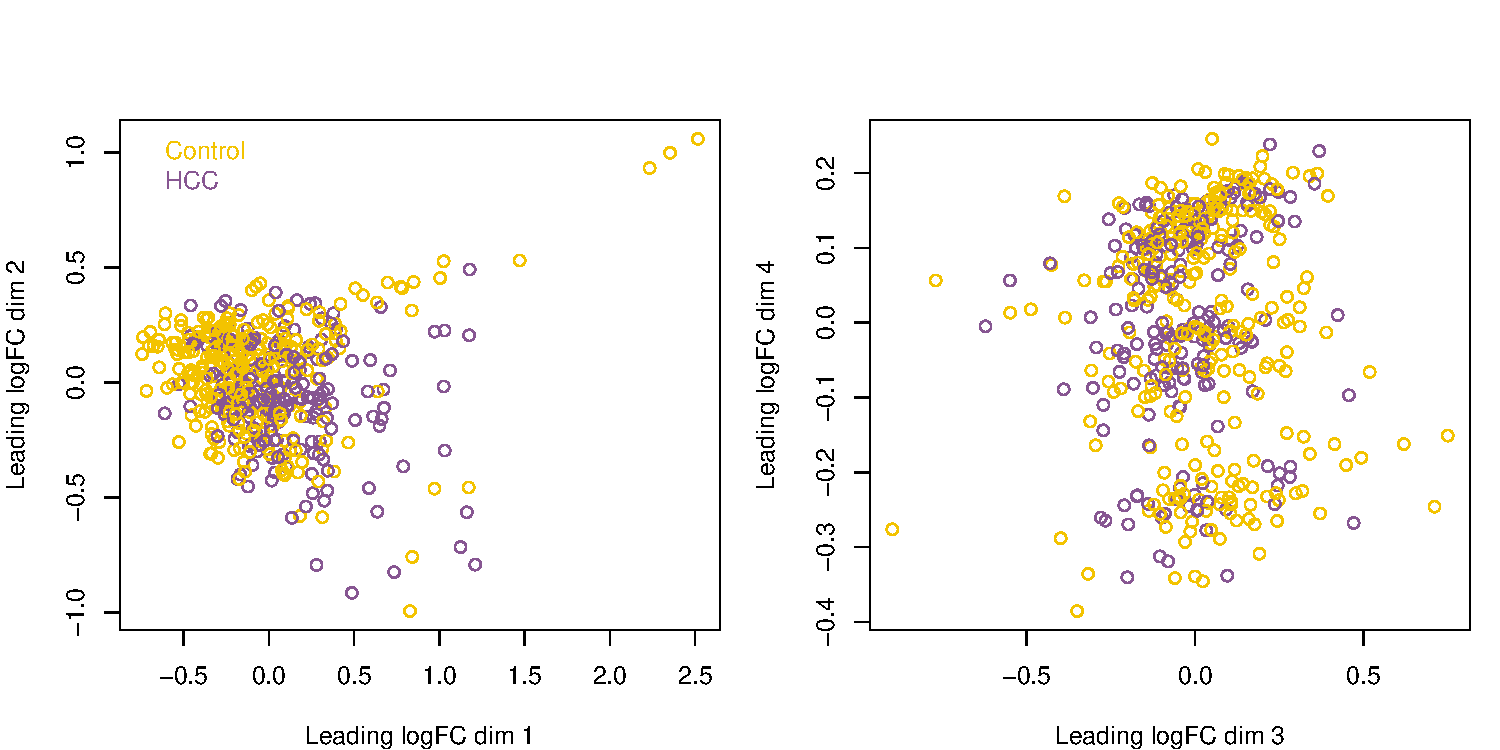
\includegraphics{HCC5hmCExplore_files/figure-latex/plotMDS-1.pdf}
\caption{\label{fig:plotMDS}MDS plots of log-CPM values}
\end{figure}

The MDS plot, which is analogous to a PCA plot adapted to gene exression data,
does not indicate strong clustering of samples. The fanning pattern observed in the
first two dimensions indicates that a few samples are drifting way from the
core set, but in no particular direction.

\hypertarget{analysis-of-coverage-variability}{%
\section{Analysis of coverage variability}\label{analysis-of-coverage-variability}}

We will use the methods described in Hart et al.~(2013) \citep{Hart:2013aa}
to characterize coverage variability in these data.
These methods do not take multiple comparisons into account.
Other tools for sample size calculation in RNA-Seq studies include
Bi and Liu (2016) \citep{Bi:2016aa}, Baccarella (2018) \citep{Baccarella:2018aa},
Guo (2014) \citep{Guo:2014aa}, Yu (2017) \citep{Yu:2017aa}, and
Zhao (2018) \citep{Zhao:2018ab}.
Poplawski (2018) \citep{Poplawski:2017aa}
evaluated RNA-seq sample size tools identified from a systematic search. They found the six evaluated tools provided widely different answers, which were strongly affected by fold change.

The references listed above aim at providing guidance for RNA-Seq experimental design.
There is much discussion and a wide range of opinion on sample size requirements
to ensure reproducibility in RNA-Seq results. At one end of the spectrum,
Ein-Dor et al.~(2006) \citep{Ein-Dor:2006aa} argue that thousands of samples are needed to
generate a robust gene list for predicting outcome in cancer. At the other end,
Dobbin et al.~(2007, 2008) \citep{Dobbin:2007aa, Dobbin:2008aa} claim that sample sizes in
the range of 20--30 per class may be adequate for building a good predictor in many cases.
Part of the disparity in sample size requirement recomendation comes from
differences of opinion in terms of what constitutes \texttt{reproducible\ results}.
In the context of sample classification, if we focus on the predicted probabilities
for individual samples, we may find good reproducibility across studies with
moderate samples sizes. If, on the other hand, we closely inspect the gene
signatures reported across studies, much greater sample sizes may be required to
achieve concordance. Kim (2009) \citep{Kim:2009aa}, like Ein-Dor et al., also find
issues in RNA-Seq research in terms of the instability of identified prognostic
gene signatures, few overlap between independently developed prognostic gene signatures, and
poor inter-study applicability of gene signatures. Fan et al.~(2006) \citep{Fan:2006aa},
on the other hand, found good concordance among gene-expression--based predictors
for breast cancer. We will return to this question when we examine
the relationship between classification model results and sample size in this
dataset later on this paper.

For two groups comparisons, the basic formula for the required number of samples per group is:

\[ n = 2(z_{1-\alpha/2} + z_{\beta})^2 \frac{(1/\mu + \sigma^2)}{ln(\Delta^2)} \]

\begin{itemize}
\tightlist
\item
  The parameters \(\alpha\) and \(\beta\) are \textbf{size} and \textbf{power} of the test.\\
\item
  \(\Delta\) is the targeted \textbf{effect size}.\\
\item
  \(\mu\) and \(\sigma\) are the \textbf{mean} and \textbf{coefficient of variation}
  of the distribution of measurement, gene representation indices in this case.
\end{itemize}

These three parameters will be fixed across genes or a given study, and are often dictated by
external requirements. Typical values might be an effect size of \(\Delta = 1.5\)
(a.k.a fold change), corresponding to detection of a 50\% change in gene expression
between the two groups.
\(z_{1 - .05/2} = 1.96\), corresponding to a two sided test at size \(\alpha = 0.05\);
and \(z_{.90}= 1.28\) corresponding to 90\% power.
The other two variables will be gene and experiment dependent: the normalized depth
of coverage \(\mu\) of the gene, and the coefficient of variation \(\sigma\) in this
gene between biological replicates. The technical variation of the
comparison is inversely proportional to the number of sequenced reads
for the gene and therefore decreases with sequencing depth.
The biological variation is a property of the particular gene/model system/condition under study.
One would expect it to be smaller for uniform systems such as cell culture and/or products that
are under tight regulatory control, and larger for less uniform replicates such
as human subject samples. The dataset under study in this report is the first of its
kind to give us an idea of variability levels in 5hmC representation.

As in Hart et al.~(2013) \citep{Hart:2013aa}
, we estimate the
biological coefficient of variation (CV) in expression across samples in the data set
using a negative binomial model.

\begin{Shaded}
\begin{Highlighting}[]
\NormalTok{ BCV\_mtx <{-}}\StringTok{ }\KeywordTok{do.call}\NormalTok{(}\StringTok{\textquotesingle{}cbind\textquotesingle{}}\NormalTok{, }\KeywordTok{lapply}\NormalTok{(}\KeywordTok{unique}\NormalTok{(sampDescA}\OperatorTok{$}\NormalTok{group), }
 \ControlFlowTok{function}\NormalTok{(GRP) \{}
\NormalTok{  GRP\_dgel <{-}}\StringTok{ }
\StringTok{    }\NormalTok{edgeR}\OperatorTok{::}\KeywordTok{DGEList}\NormalTok{(}\DataTypeTok{counts=}\NormalTok{featureCountsA[, sampDescA}\OperatorTok{$}\NormalTok{group}\OperatorTok{==}\NormalTok{GRP])}
\NormalTok{  GRP\_dgel <{-}}\StringTok{ }\NormalTok{edgeR}\OperatorTok{::}\KeywordTok{estimateDisp}\NormalTok{(GRP\_dgel)}

  \KeywordTok{sqrt}\NormalTok{(GRP\_dgel}\OperatorTok{$}\NormalTok{tagwise.dispersion)}
\NormalTok{  \}))}
\end{Highlighting}
\end{Shaded}

\begin{verbatim}
## Design matrix not provided. Switch to the classic mode.
## Design matrix not provided. Switch to the classic mode.
\end{verbatim}

\begin{Shaded}
\begin{Highlighting}[]
 \KeywordTok{colnames}\NormalTok{(BCV\_mtx) <{-}}\StringTok{ }\KeywordTok{unique}\NormalTok{(sampDescA}\OperatorTok{$}\NormalTok{group)}
 \KeywordTok{plot}\NormalTok{(spatstat}\OperatorTok{::}\KeywordTok{CDF}\NormalTok{(}\KeywordTok{density}\NormalTok{(BCV\_mtx[,}\DecValTok{1}\NormalTok{])), }
   \DataTypeTok{col=}\NormalTok{groupCol[}\KeywordTok{colnames}\NormalTok{(BCV\_mtx)[}\DecValTok{1}\NormalTok{]], }
   \DataTypeTok{lwd=}\DecValTok{2}\NormalTok{, }\DataTypeTok{ylab=}\StringTok{\textquotesingle{}Prob(BCV<x)\textquotesingle{}}\NormalTok{,}
   \DataTypeTok{xlim=}\KeywordTok{c}\NormalTok{(}\DecValTok{0}\NormalTok{, }\FloatTok{0.5}\NormalTok{))}
 \ControlFlowTok{for}\NormalTok{(JJ }\ControlFlowTok{in} \DecValTok{2}\OperatorTok{:}\KeywordTok{ncol}\NormalTok{(BCV\_mtx))}
 \KeywordTok{plot}\NormalTok{(spatstat}\OperatorTok{::}\KeywordTok{CDF}\NormalTok{(}\KeywordTok{density}\NormalTok{(BCV\_mtx[,JJ])), }
   \DataTypeTok{col=}\NormalTok{groupCol[}\KeywordTok{colnames}\NormalTok{(BCV\_mtx)[JJ]], }
   \DataTypeTok{lwd=}\DecValTok{2}\NormalTok{, }\DataTypeTok{add=}\NormalTok{T, }\DataTypeTok{xlim=}\KeywordTok{c}\NormalTok{(}\DecValTok{0}\NormalTok{, }\FloatTok{2.0}\NormalTok{))}
 \KeywordTok{legend}\NormalTok{(}\StringTok{\textquotesingle{}bottomright\textquotesingle{}}\NormalTok{, }\DataTypeTok{legend=}\KeywordTok{names}\NormalTok{(groupCol), }\DataTypeTok{col=}\NormalTok{groupCol, }\DataTypeTok{lwd=}\DecValTok{2}\NormalTok{)}
\NormalTok{ BCV\_90perc\_vec <{-}}\StringTok{ }\KeywordTok{round}\NormalTok{(}\KeywordTok{apply}\NormalTok{(BCV\_mtx,}\DecValTok{2}\NormalTok{,quantile, }\DataTypeTok{prob=}\FloatTok{0.90}\NormalTok{), }\DecValTok{2}\NormalTok{)}
\NormalTok{ BCV\_50perc\_vec <{-}}\StringTok{ }\KeywordTok{round}\NormalTok{(}\KeywordTok{apply}\NormalTok{(BCV\_mtx,}\DecValTok{2}\NormalTok{,quantile, }\DataTypeTok{prob=}\FloatTok{0.50}\NormalTok{), }\DecValTok{2}\NormalTok{)}
 \ControlFlowTok{for}\NormalTok{(JJ }\ControlFlowTok{in} \DecValTok{1}\OperatorTok{:}\KeywordTok{length}\NormalTok{(BCV\_90perc\_vec)) }
 \KeywordTok{rug}\NormalTok{(BCV\_90perc\_vec[JJ], }\DataTypeTok{lwd=}\DecValTok{2}\NormalTok{, }\DataTypeTok{ticksize =} \FloatTok{0.05}\NormalTok{,}
    \DataTypeTok{col=}\NormalTok{groupCol[}\KeywordTok{names}\NormalTok{(BCV\_90perc\_vec)[JJ]])}
\end{Highlighting}
\end{Shaded}

\begin{figure}
\centering
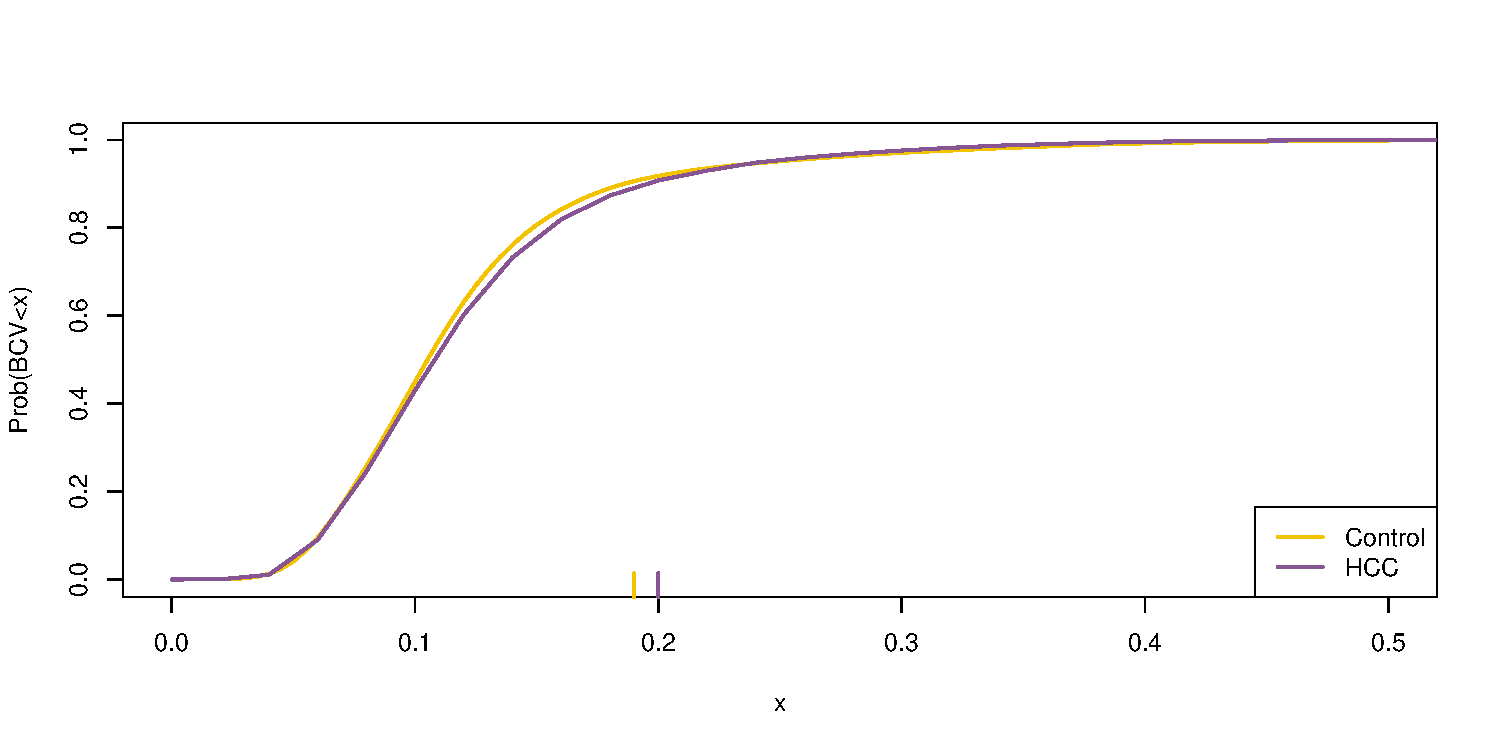
\includegraphics{HCC5hmCExplore_files/figure-latex/estBCV-1.pdf}
\caption{\label{fig:estBCV}Cumulative Distribution of CV - rug = 90th percentile}
\end{figure}

We can now look at sample size estimates to required to detect
various effect sizes. The effect sizes examined here are selected
based on the differential representation analysis in Section \ref{dra} below.

\begin{Shaded}
\begin{Highlighting}[]
\KeywordTok{par}\NormalTok{(}\DataTypeTok{mfrow =} \KeywordTok{c}\NormalTok{(}\DecValTok{2}\NormalTok{, }\DecValTok{1}\NormalTok{), }\DataTypeTok{mar =} \KeywordTok{c}\NormalTok{(}\DecValTok{3}\NormalTok{, }\DecValTok{3}\NormalTok{, }\DecValTok{2}\NormalTok{, }\DecValTok{1}\NormalTok{), }\DataTypeTok{oma =} \KeywordTok{c}\NormalTok{(}\DecValTok{2}\NormalTok{, }\DecValTok{2}\NormalTok{, }\DecValTok{2}\NormalTok{, }\DecValTok{0}\NormalTok{))}
\ControlFlowTok{for}\NormalTok{ (EFFECT }\ControlFlowTok{in} \KeywordTok{c}\NormalTok{(}\FloatTok{1.10}\NormalTok{, }\FloatTok{1.20}\NormalTok{)) \{}
  \KeywordTok{plot}\NormalTok{(}
    \DataTypeTok{x =} \DecValTok{10}\OperatorTok{:}\DecValTok{100}\NormalTok{, }
    \DataTypeTok{y =}\NormalTok{ RNASeqPower}\OperatorTok{::}\KeywordTok{rnapower}\NormalTok{(}\DataTypeTok{depth =} \DecValTok{10}\OperatorTok{:}\DecValTok{100}\NormalTok{, }\DataTypeTok{cv =} \KeywordTok{max}\NormalTok{(BCV\_90perc\_vec), }
         \DataTypeTok{effect =}\NormalTok{ EFFECT, }\DataTypeTok{alpha =} \FloatTok{.05}\NormalTok{, }\DataTypeTok{power =} \FloatTok{.80}\NormalTok{),}
    \DataTypeTok{lwd =} \DecValTok{2}\NormalTok{, }\DataTypeTok{ylab =} \StringTok{""}\NormalTok{, }\DataTypeTok{xlab =} \StringTok{""}\NormalTok{, }\DataTypeTok{type=}\StringTok{\textquotesingle{}l\textquotesingle{}}
\NormalTok{  )}
  \KeywordTok{title}\NormalTok{(}\KeywordTok{paste}\NormalTok{(}\StringTok{"Effect ="}\NormalTok{, EFFECT, }\StringTok{"cv ="}\NormalTok{, }
     \KeywordTok{max}\NormalTok{(BCV\_90perc\_vec), }\StringTok{"Alpha=0.05, Beta=0.80"}\NormalTok{))}
\NormalTok{\}}
\KeywordTok{mtext}\NormalTok{(}\DataTypeTok{side =} \DecValTok{1}\NormalTok{, }\DataTypeTok{outer =}\NormalTok{ T, }\StringTok{"Gene Coverage"}\NormalTok{)}
\KeywordTok{mtext}\NormalTok{(}\DataTypeTok{side =} \DecValTok{2}\NormalTok{, }\DataTypeTok{outer =}\NormalTok{ T, }\StringTok{"Samples Needed"}\NormalTok{)}
\KeywordTok{mtext}\NormalTok{(}\DataTypeTok{side =} \DecValTok{3}\NormalTok{, }\DataTypeTok{outer =}\NormalTok{ T, }\DataTypeTok{cex =} \FloatTok{1.25}\NormalTok{, }
    \StringTok{"Negative Binomial 2 Group Sample Size Curves"}\NormalTok{)}
\end{Highlighting}
\end{Shaded}

\begin{figure}
\centering
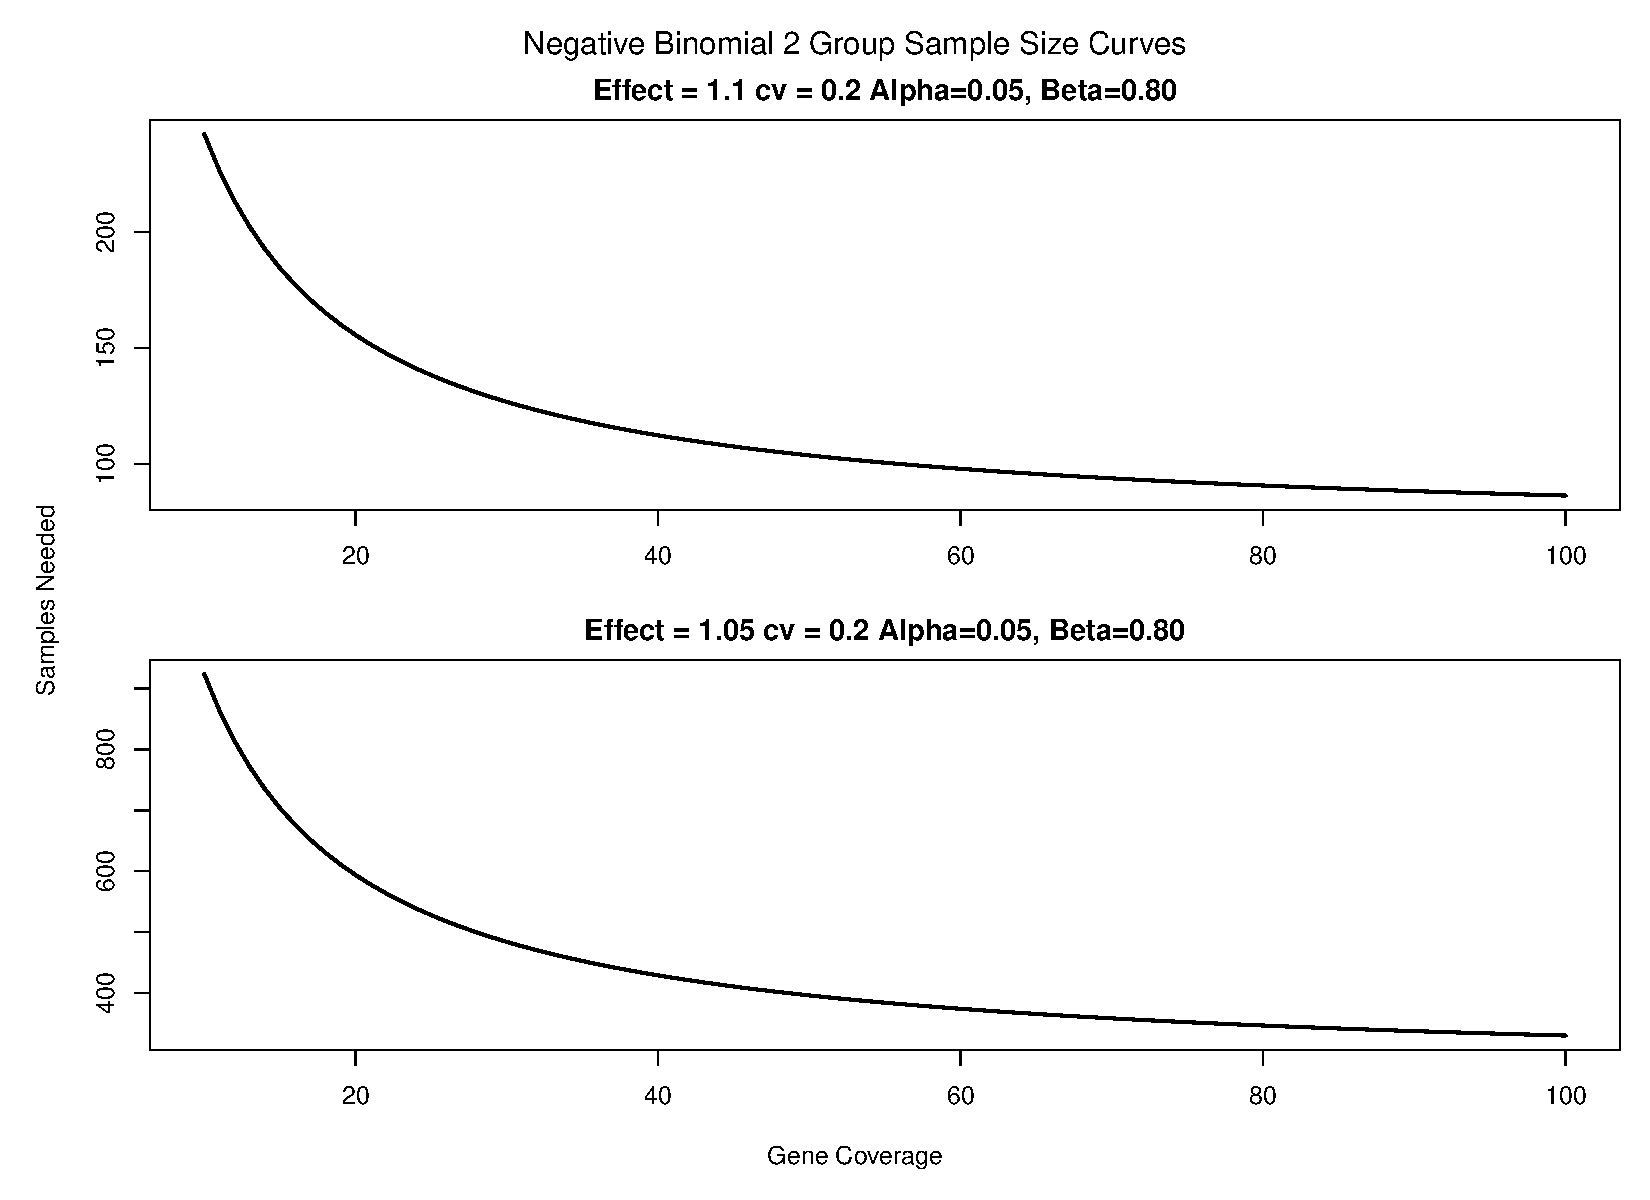
\includegraphics{HCC5hmCExplore_files/figure-latex/sampleSizeCurve-1.pdf}
\caption{\label{fig:sampleSizeCurve}Sample Size Estimates}
\end{figure}

Note that with these data, moderate sample sizes are adequate
to detect genes with an effect size of 1.2 (20\% fold change). This is due to the fact
that the biological variability in gene body 5hmC density is quite low.
For human samples, RNA-Seq within group biological variability is
typically in the 0.4-1.0 range \citep{Hart:2013aa}.

\hypertarget{dra}{%
\section{Differential representation analysis}\label{dra}}

\begin{itemize}
\tightlist
\item
  word on GC content
\end{itemize}

\hypertarget{baseline-model}{%
\chapter{Baseline Model}\label{baseline-model}}

In the section we look at the baseline model fit:

\begin{itemize}
\item
  What is the accuracy?\\
\item
  Look at individual points and store some sample scores
\item
  Baseline model

  \begin{itemize}
  \tightlist
  \item
    how separable are the data
  \item
    individual sample quality
  \end{itemize}
\end{itemize}

\hypertarget{model-suite}{%
\chapter{Fitted Model Suite}\label{model-suite}}

We examine the results of fitting a suite of models to
investigate the effect of sample size on model performance.

\hypertarget{conclusions}{%
\chapter{Conclusions}\label{conclusions}}

We have found that \ldots{}

Other questions \ldots{}

  \bibliography{bib/HCC5hmc.bib}

\end{document}
